\newcommand{\secondLanguage}{icelandic} 			% if a second language is used, add it here
\documentclass[draft, {\secondLanguage}, english]{volcanica-template} 
\nonstopmode									% can toggle to see compilation warnings
\newcommand{\ArticleType}{Report}			
% Please choose between Research article, Report, Review, or Methods. 
% Details about different article types are available at: 
% https://www.jvolcanica.org/ojs/index.php/volcanica/about/submissions

%------------------------------------------------------------
%  Article details go here 
%------------------------------------------------------------	
\newcommand{\Title}{AI for Sustainable Agriculture and for Drinking Water Grids} 	% Manuscript title goes here.
\newcommand{\shortTitle}{AI for SDGs} 		        % Short title for header goes here, less than 60 characters.
\newcommand{\Author}{P.Tahan A.Maci\xspace}    	% First author goes here.

%------------------------------------------------------------
%  Author details go here 
%------------------------------------------------------------	
\author[{{\affiliation{1}}}] 				% affiliation number
{\orcidaffil{0000.0000.0000.0000}~			% orcid number
Paria Tahan	 				% first author
\Email{paria.tahan@studenti.unipd.it}} 		        	% corresponding author email
\author[{{\affiliation{2}}}] 				% affiliation number
{\orcidaffil{0000.0000.0000.0000}~			% orcid number
Andrea Maci 			
\Email{andrea.maci@studenti.unipd.it}} 		% second author

%------------------------------------------------------------
%  Affiliations 		
%------------------------------------------------------------	
\affil[{{\affiliation{1}}}]{					% affiliation #1
2043889 paria.tahan@studenti.unipd.it; Department of Computer Engineering.
}
\affil[{{\affiliation{2}}}]{					% affiliation #2
2063146 andrea.maci@studenti.unipd.it; Department of Computer Engineering.
}

%------------------------------------------------------------
%  BIBLIOGRAPHY FILE 		
%------------------------------------------------------------	  
\addbibresource{bib-file.bib}		  		% add the name of the bibliography file here

%------------------------------------------------------------
%  Start of Document 		
%------------------------------------------------------------	  
\begin{document}

%------------------------------------------------------------
%  Abstract(s) and Keywords
%------------------------------------------------------------	
% Replace dummy text (\protect{\lipsum[45]}) with the abstract in the first argument for \FrontMatter (between the curly braces {}). 
% If there is a second-language abstract, it goes between the square brackets []. 
% Make sure you have included the correct language in line 1, above.
% If no second abstract, ensure there is no space between the square brackets [].
\FrontMatter{\protect{This report discusses two recent papers published in the book The Ethics
of Artificial Intelligence for the Sustainable Development Goals. One belongs to the use of artificial intelligence (AI) to promote sustainable agriculture and rangeland monitoring. AI can be used to improve crop yields, reduce water usage, and enhance soil health, among other benefits. The paper also examines the challenges associated with implementing AI in agriculture and rangeland management, such as the need for accurate data and the potential for unintended consequences. The other paper focuses on the use of the Internet of Things (IoT) to improve the control of drinking water grids. The paper proposes a system that uses IoT devices to monitor the water supply and demand in real time and then uses this data to optimize the operation of the water grid. The paper discusses the benefits of this approach, including improved water quality and reduced waste, and also addresses the challenges associated with implementing such a system, such as the need for secure data transmission and the potential for system failures.}}
[]% 
{
\keywords{AI}{Climate change}{Agricultural management}{Rangeland monitoring}{Sustainable Development Goals}{Water}{Leak detection}{WSN}{Quality}{Monitoring}	% add up to six keywords in curly braces {}
}

%------------------------------------------------------------
%  Maintext
%------------------------------------------------------------	
%\hypertarget{introduction}{%
%\section{Introduction}\label{introduction}}		
%In this section, a brief description of the report will be explained. Section 2 will be dedicated to the paper "AI for Sustainable Agriculture and Rangeland Monitoring". the section contains subsections giving information about the problem overview and explaining the SGDs target indicators. Then we will talk about the background of Rangelands and the application of AI for climate change and agriculture. in the next subsection, the proposed method will be described with the data that is used in the research. Finally, the section will be finished with the discussion and conclusion.

%In Section 3, the report talks about "Smart Control of Drinking Water Grids Using IoT". After giving the problem overview and previous related works the proposed architecture will be explained. The report will be continued by introducing a model for Water Quality Analysis Based on Machine Learning and how is the processing of data gathering and aggregation. next subsections explain more about the classification with machine learning algorithms. After that is time to talk about the experiments and finally the paper conclusion.

\section{AI for Sustainable Agriculture and Rangeland Monitoring}\label{sec:02}
This paper \parencite{Efremova2023} explores the use of AI and satellite imagery in sustainable agriculture for resource allocation based on satellite monitoring results. A novel framework is proposed, incorporating AI and earth observation data, to address climate change-related challenges in the agri-food sector.

A case study involving a conservancy examines resource allocation decisions for optimal grazing and soil nutrition using cattle herds. Physical biomonitoring parameters are monitored through satellite imagery, and an AI-based approach is proposed for efficient interpretation. The results indicate that the framework enables real-time monitoring with accurate biomonitoring estimations and improved resource allocation practices aligned with SDG 2 \parencite{Efremova2023}.

\subsection{Problem Overview}\label{sec:02a}
The combination of AI and earth observation data can enhance the monitoring of Sustainable Development Goals (SDGs) and provide an efficient means of monitoring crops, livestock, and rangelands in agriculture and rangeland management. However, challenges such as accurate and reliable data, tailored AI algorithms, and ethical and social issues must be addressed to ensure that AI benefits farmers, ranchers, and the environment. By addressing these challenges, AI has the potential to support sustainable agriculture and rangeland management and contribute to achieving the United Nations' Sustainable Development Goals despite the challenges posed by population growth, climate change, and environmental pressures.

\subsubsection{AI-EO SDG Model: Zero Hunger}\label{sec:02aa}
Despite progress in reducing hunger and malnutrition, the problem still persists, particularly in sub-Saharan Africa and South Asia, and has been worsened by the COVID-19 pandemic. The issue is complex and influenced by various factors. To address it, a multi-faceted approach is required, integrating interventions such as increasing agricultural productivity, improving access to nutritious foods, strengthening social safety nets, and promoting gender equality. The AI-EO Model aims to support evidence-based decision-making and monitoring of progress toward zero hunger by utilizing artificial intelligence and Earth observation data.

\subsubsection{AI-EO SDG Model: Climate Change}\label{sec:02ab}
Climate change is a pressing global challenge, with severe impacts already being felt in various sectors. The issue is complex and caused by human activities such as burning fossil fuels and deforestation. Addressing it requires a multi-faceted approach that involves reducing greenhouse gas emissions, building resilience, and transitioning to a more sustainable and low-carbon economy. The AI-EO SDG Model aims to support the decision-making and monitoring of progress towards mitigating and adapting to climate change, as well as addressing the issue of hunger and malnutrition.

\subsection{Background}\label{sec:02b}
\subsubsection{Rangelands}\label{sec:02ba}
Rangelands are natural landscapes that are used for grazing livestock and provide important ecosystem services, such as carbon storage, water regulation, and biodiversity conservation. Rangelands cover a significant portion of the Earth's land surface, with an estimated 25\% of the world's land area classified as rangelands. However, rangelands are under increasing pressure from a range of factors, including climate change, land use change, and overgrazing, which can lead to soil degradation, loss of biodiversity, and reduced capacity to sequester carbon.

The challenges facing rangelands require a multi-faceted approach that incorporates a range of interventions, from improving livestock management practices and reducing overgrazing to promoting sustainable land use practices and restoring degraded ecosystems. 

\subsubsection{AI for Climate Change and Agriculture: Overview}\label{sec:02bb}
AI has the potential to support decision-making and enhance the efficiency and effectiveness of agricultural systems, by providing insights into weather patterns, crop growth, and soil health. AI can also be used to develop predictive models of climate change impacts, identify areas at risk of soil erosion and degradation, and improve the efficiency of irrigation systems.

AI has applications in agriculture, including precision agriculture, which uses sensors and machine learning algorithms to optimize crop yields while reducing inputs such as water and fertilizer. Another application is the use of AI in supporting climate-smart agriculture, which seeks to promote sustainable land use practices that reduce greenhouse gas emissions, enhance the resilience of agricultural systems to climate change, and increase the productivity and income of smallholder farmers.

\subsection{Methods}\label{sec:02c}
\subsubsection{Overview of the Proposed Approach}\label{sec:02ca}
The AI-EO model will be designed to integrate artificial intelligence and Earth observation data to support decision-making and monitoring of progress toward the goal of climate change mitigation and adaptation. 

Key components of the proposed approach, include the development of machine learning algorithms to analyze large volumes of Earth observation data and generate actionable insights for decision-makers. These algorithms will be trained on historical data and will use a range of techniques, such as deep learning and neural networks, to identify patterns and trends in the data. The model will incorporate climate models to develop predictive models of climate change impacts, which can be used to inform decision-making and support climate adaptation strategies.

It's important to incorporate socio-economic data into the AI-EO SDG Model to understand climate change's human dimensions and support climate-smart policies. This requires integrating data on factors such as population density, land use patterns, and economic activity to identify vulnerable populations and areas at risk of climate change impacts. The model should be flexible and scalable, adaptable to different contexts and used by policymakers to farmers. Overall, the AI-EO SDG Model aims to provide decision-makers with a comprehensive understanding of human and natural systems to support sustainable development.

\subsubsection{Data}\label{sec:02cb}
The importance of Earth observation data in providing information on key environmental indicators, such as land cover, vegetation indices, and soil moisture. This data can be used to monitor changes in the environment, identify areas at risk of degradation, and support the development of climate-smart land use policies.  The importance of climate models in developing predictive models of climate change impacts, which can be used to inform decision-making and support climate adaptation strategies also should be emphasized.

\subsubsection{Model Architecture}\label{sec:02cc}

%\begin{figure*}[!t]								%[tbhp]
%\centering
%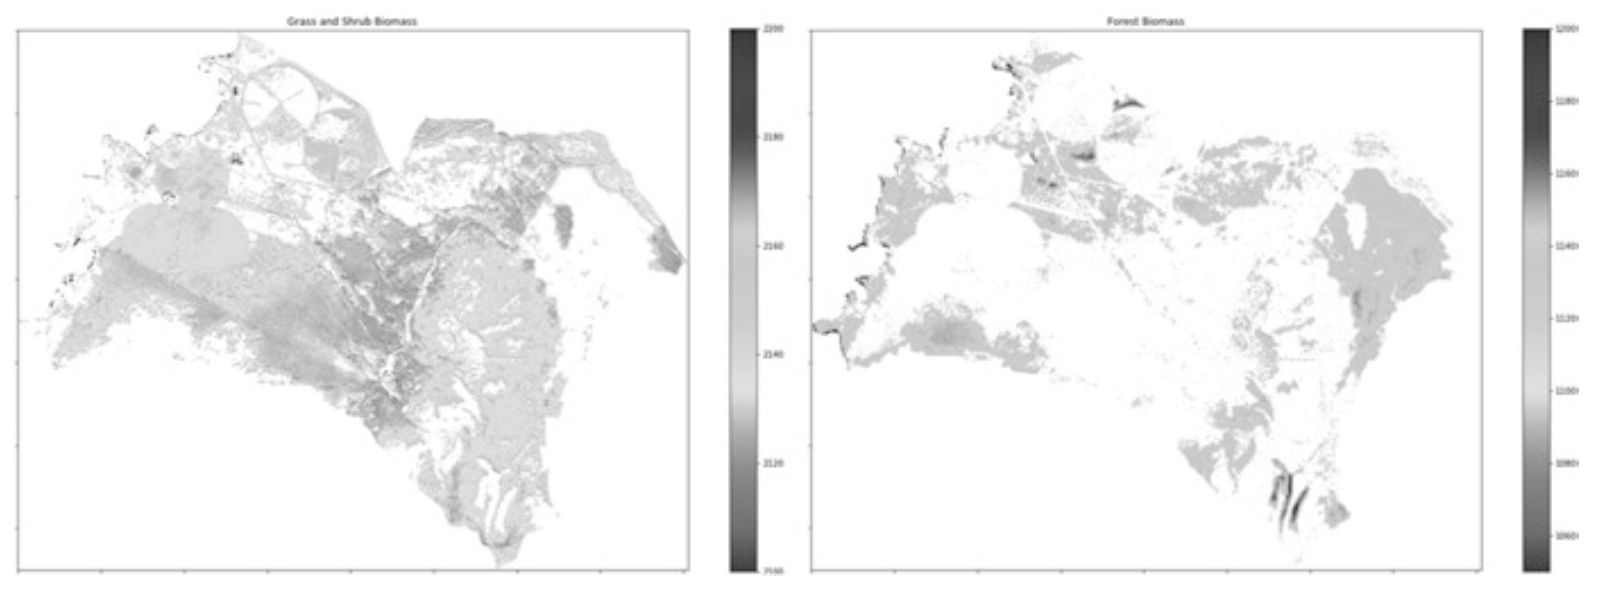
\includegraphics[width=\textwidth]{Images/fig1-3.png}
%\caption{Biomass estimation for grassland, shrublands, and forest land cover types}	
%\label{fig:01}									
%\end{figure*}

The paper describes the three main modules that will make up the model architecture: the data processing module, the feature extraction module, and the predictive modeling module. The data processing module will be responsible for pre-processing and cleaning the data and will include functions for ingesting data from a range of sources, such as satellite sensors, climate models, and socio-economic databases. The module will also include tools for data quality control, data normalization, and data transformation, in order to ensure that the data is accurate, reliable, and consistent. The feature extraction module will be responsible for identifying relevant features and patterns in the data, using a range of techniques such as machine learning algorithms and statistical analyses. The module will also include tools for feature selection, feature engineering, and dimensionality reduction, in order to reduce the complexity of the data and improve the efficiency of the predictive modeling module.

The predictive modeling module will be responsible for developing machine learning algorithms that can generate actionable insights from the data. The module will use a range of techniques, such as deep learning, neural networks, and decision trees, to generate models that can predict key outcomes related to climate change, such as changes in temperature, precipitation, or vegetation cover. The module will also incorporate uncertainty and sensitivity analyses, in order to provide decision-makers with a range of possible scenarios and their associated risks and opportunities.

The proposed model architecture consists of several crucial sub-modules that will be integrated to form a comprehensive framework. One such sub-module is the data integration and fusion component, which will handle the integration and fusion of data from diverse sources. Its purpose is to provide a unified understanding of the intricate interactions between human and natural systems. This sub-module will incorporate tools for data mapping, harmonization, and fusion to ensure data consistency and standardization across various sources.

Another essential sub-module is the feedback and evaluation component, which will assess the model's performance and incorporate user feedback during the model development process. It will encompass tools for model validation, comparison, and improvement, ensuring the accuracy, reliability, and relevance of the model to decision-makers. By employing a modular architecture, the AI-EO SDG Model for Climate Change aims to offer a flexible and scalable framework. This approach enables the incorporation of new data sources and modules as they become available and facilitates adaptation to different contexts, catering to the needs of diverse stakeholders, including policymakers, farmers, and land managers.

%\begin{figure*}[!t]								%[tbhp]
%\centering
%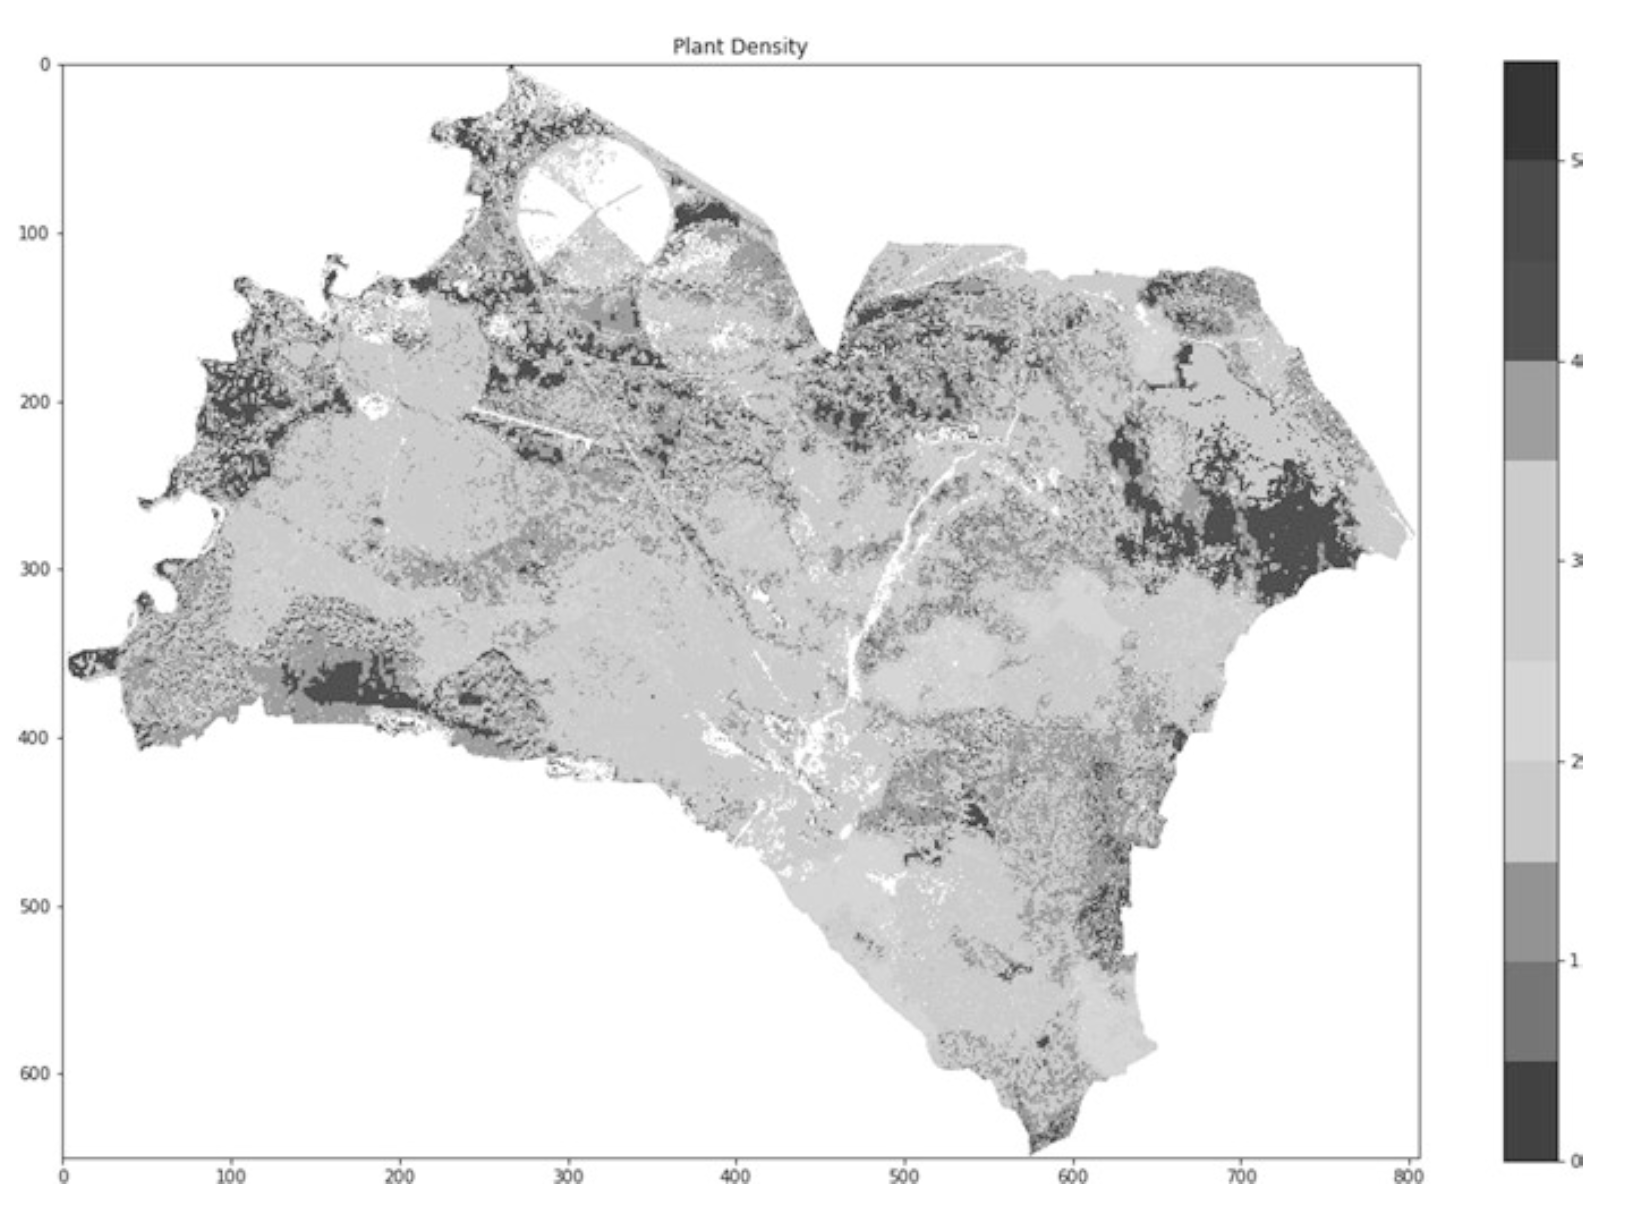
\includegraphics[width=\textwidth]{Images/fig2-3.png} 
%\caption{Estimation of plant density across the rangelands. The colour coding shows the highest vegetation areas as blue and the lowest as red, respectively
%}	
%\label{fig:02}									
%\end{figure*}

In addition to the three main modules, there are other important sub-modules that will be integrated into the model architecture. These include the sensor calibration and validation sub-module, which will be responsible for ensuring the accuracy and reliability of the satellite sensors used to collect Earth observation data. The sub-module will include tools for sensor calibration, sensor validation, and data quality control, in order to ensure that the data is accurate and reliable.

Another important sub-module is the data visualization and communication sub-module, which will be responsible for presenting the data and the insights generated by the model in a clear and understandable way. The sub-module will include tools for data visualization, data exploration, and data communication, in order to enable decision-makers to understand the implications of the data and the insights generated by the model.

%\begin{figure*}[!t]								%[tbhp]
%\centering
%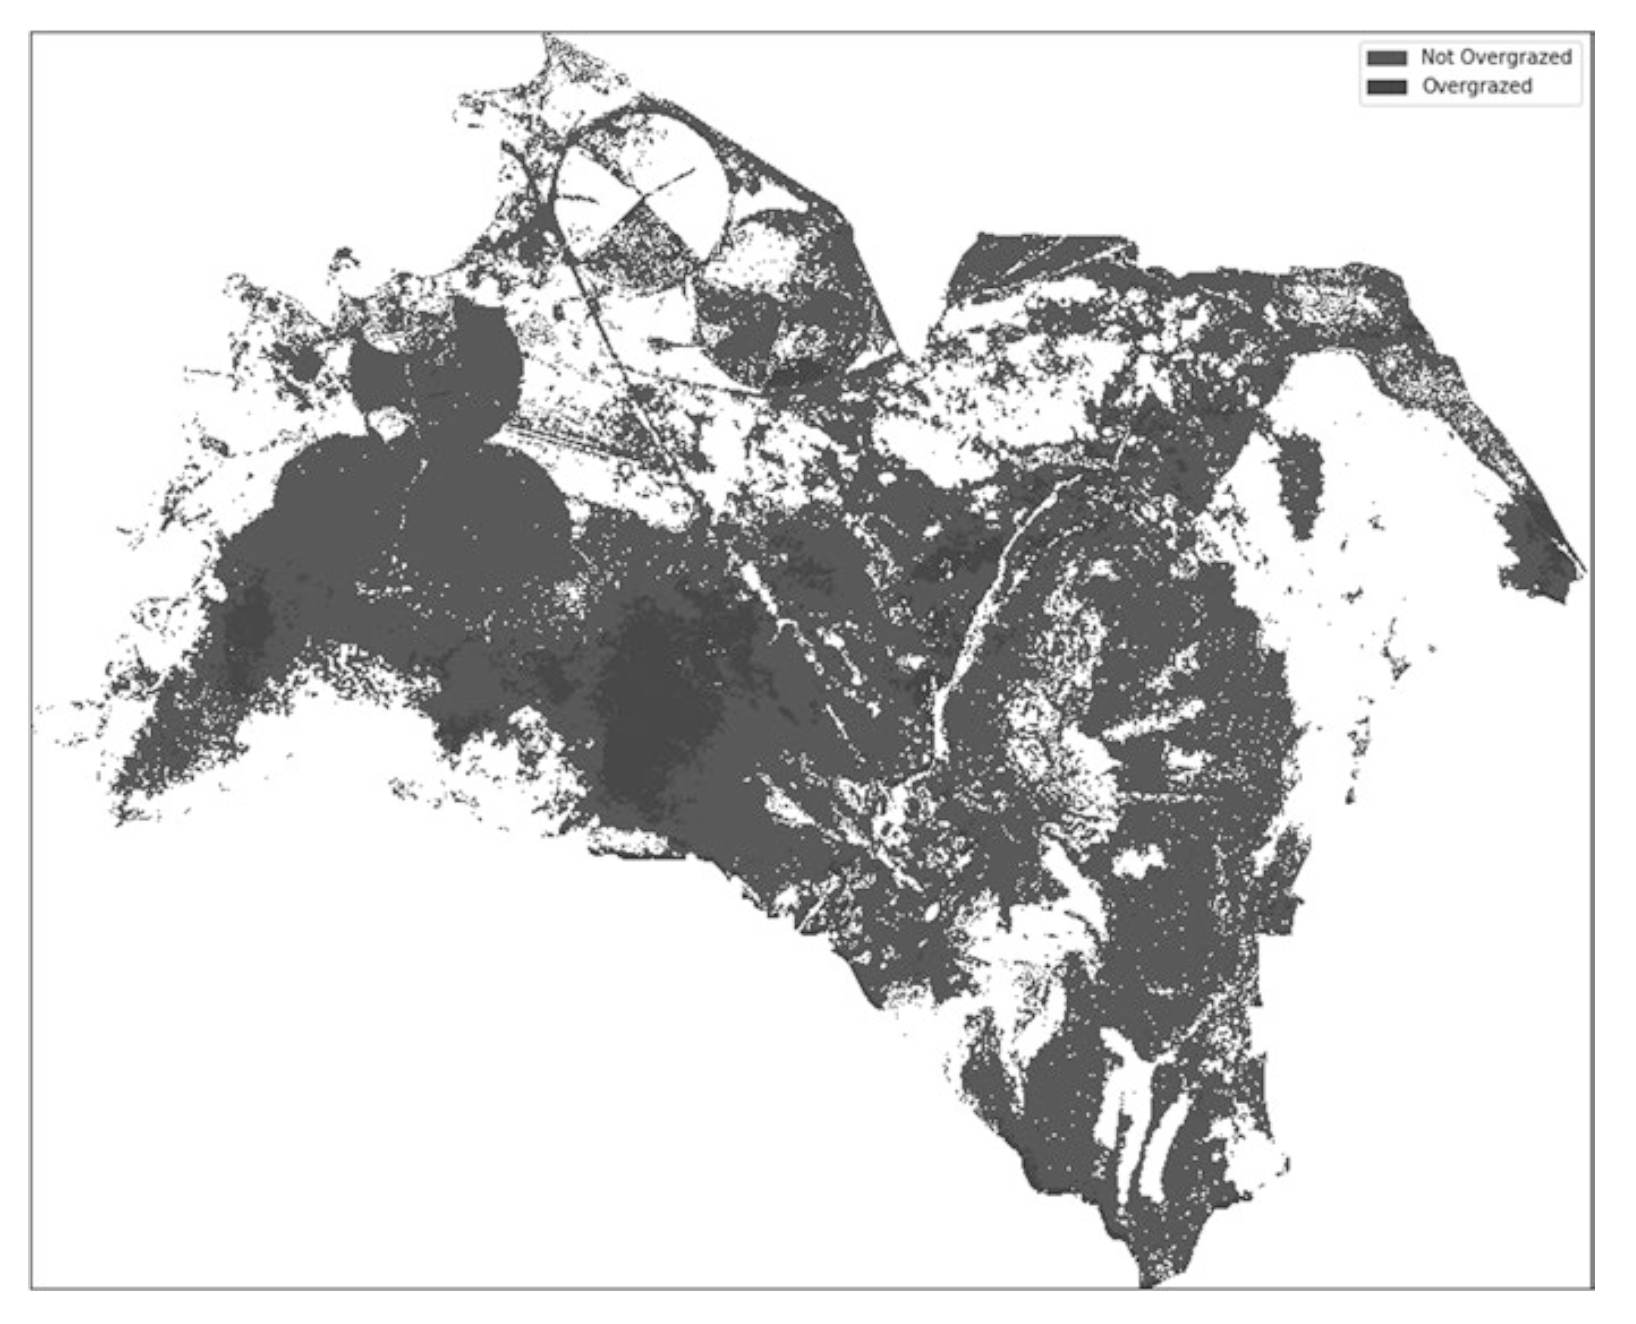
\includegraphics[width=\textwidth]{Images/fig3-3.png} 
%\caption{Overgrazing prediction. Red areas indicate the places with the highest degrees of overgrazing}	
%\label{fig:03}									
%\end{figure*}

The AI models developed in this study surpassed the performance of state-of-the-art models. The land cover segmentation task achieved an accuracy of 79 \%, with training, validation, and test loss values of 0.32, 0.1, and 0.79, respectively. However, the model showed some confusion between agricultural land and bare soil, possibly due to the bare state of agricultural land after crop harvesting. The biomass parameter was also accurately predicted, with a training accuracy of 98 \% and a testing accuracy of 97 \% on biomass measures. The model outperformed similar studies in biomass estimation using the same or lower resolution imagery.

The parameters classified into 0-5 quantiles had varying accuracy depending on the parameter, with errors generally ranging from 0.5-1 due to the discrete ordinal nature of the classes. Each parameter had a different mean error and error distribution. The overgrazing parameter, which is crucial for conservancy management decisions about moving cattle, had a training accuracy of 98 \% and a testing accuracy of 86 \% with 84 \% accuracy for overgrazed pixels and 92 \% accuracy for non-overgrazed pixels. The model predicted overgrazing across all grass and shrub areas, creating a binary image of either overgrazed or not overgrazed pixels.

The high accuracy achieved by the model indicates its potential for real-life monitoring applications. The resulting errors in the measurements are considered negligible, making the model useful for managerial decisions related to land management, such as moving cattle or optimizing grazing practices. Overall, the proposed approach outperforms similar studies in biomass estimation using the same or lower resolution imagery, highlighting its potential for practical use in land management decision-making.

Finally, the model architecture will incorporate a cloud-based infrastructure, which will enable the model to be easily accessed and used by a wide range of stakeholders. The infrastructure will include tools for data storage, data sharing, and data analysis, and will be designed to be scalable and secure, in order to ensure the privacy and security of the data. The cloud-based infrastructure will enable the model to be easily scaled up or down, depending on the needs of users, and will enable the model to be accessed from anywhere in the world, using a range of devices.

It is concluded that the AI-EO SDG Model for Climate Change has the potential to make a significant contribution to the global effort to address the challenge of climate change, by providing decision-makers with a comprehensive and integrated understanding of the complex interactions between human and natural systems.

%\begin{figure*}[!t]								%[tbhp]
%\centering
%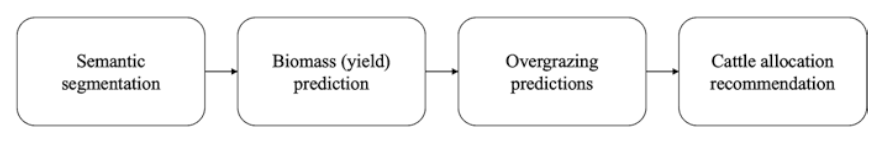
\includegraphics[width=\textwidth]{Images/fig4-3.png} 
%\caption{Model implementation for efficient resource allocation}	
%\label{fig:04}									
%\end{figure*}

\subsubsection{Challenges and Economic Implications}
One of the main challenges will be the availability and accessibility of data, particularly in developing countries, where data infrastructure may be limited. The need for capacity building and technical training to enable decision-makers to effectively use the model and interpret the insights it generates. In terms of economic implications, the model has the potential to generate significant economic benefits, particularly in the agricultural sector, by enabling farmers to make more informed decisions and improve their yields. However, the model may have implementation costs, particularly related to data processing and storage, and note that these costs will need to be carefully considered when planning for the implementation of the model.

\subsubsection{Economic Outcomes}
The provided model has the potential to generate significant economic benefits, particularly in the agricultural sector, by enabling farmers to make more informed decisions and improve their yields. In addition, it is also mentioned that the model has the potential to support the development of new climate-smart technologies and services, such as improved weather forecasting and water management systems, which can create new business opportunities and drive economic growth. However, the model may also have implementation costs, particularly related to data processing and storage, and these costs will need to be carefully considered when planning for the implementation of the model. 

\section{Smart Control of Drinking Water Grids Using IoT}
In the second paper by \cite{Dziri2023}, the authors discuss the application of Internet of Things (IoT) technology in the smart control of drinking water grids. The authors begin by discussing the importance of water, particularly in relation to human life and the challenges associated with maintaining its quality. Water is in fact a vital chemical component for life and its significance continues to increase with the needs of modern civilization. Poor water supply and sanitation conditions, especially in developing countries, contributes to approximately 80\% of the total diseases. The article highlights how IoT can revolutionize the management and monitoring of water distribution systems by providing real-time data and enabling efficient control and optimization of operations, as opposed to traditional slow and inefficient methods.

\subsection{Problem Overview}
The conventional methods of monitoring water quality involve manual collection of samples, which are then tested in laboratories. However, this approach is deemed inefficient, expensive, time-consuming, and lacks real-time results. To address this, the paper suggests the use of wireless sensor networks (WSNs) for continuous monitoring of drinking water quality. WSNs are self-configuring networks consisting of small sensor nodes that communicate with each other through radio signals. They are deployed to monitor physical or environmental conditions and transmit data to a central location for analysis. However, WSNs face challenges such as resource constraints, unreliable communication links, and low data rates. As a result, new protocols and algorithms have been developed specifically for WSN environments. The purpose of the work is to create an intelligent system for monitoring the quality of distributed drinking water, using a WSN to detect real-time contamination in the water distribution network and to address the issue of leaks in water pipes.

\subsubsection{Related works}
Before diving into the proposed architecture, the authors mention the importance of previous works in the literature, splitting them in two categories: those who focus on the monitoring of drinking water quality and those who focus on controlling leaks in water pipes.

\subsubsection{Water Quality Monitoring Systems}
Several systems for monitoring water quality have been developed. One possible system requires to measure the quality based on pH, water turbidity and temperature sensors; this is a practical and economical solution to monitor the water quality, especially in rural areas.
Another system instead exploits an IoT-based solution. This system provides remote monitoring of water quality along with water flow control via mobile application. The system classifies water quality using machine learning algorithms such as support vector machines (SVM) and deep learning neural networks.
A WSN based solution proposes to gather data about the water through pH, oxygen density and turbidity sensors. The sensors are powered by a solar power module, while the node to base station communication is realized via WSN technology.

\subsubsection{Leak Detection Solutions in the Water Distribution Network}
There are two main systems to detect leaks in water pipes. A static detection system relies on sensors and data collectors that are placed in the water distribution network. This data is periodically sent to the network management center to discover possible leaks. A dynamic detection system relies on the mobility of leak detection devices to an area where there is a suspected leak to conduct an investigation. The first system is prone to false alarms, while the latter immediately locates a leak under the assumption of already knowing the possibility of a leak. Acoustic technologies are the most commonly used in these systems. Other possible techniques involve time domain reflectometry (TDR), ground-penetrating radar (GPR), and electrical resistivity tomography (ERT), experimented in underground pipes. Novel techniques utilizing machine learning and advanced statistical methods have been recently developed for the detection and location of leaks.

\subsection{The Proposed System Architecture}
The proposed architecture develops a real-time system that monitors the water quality according to physicochemical and microbiological parameters, plus the system uses a data aggregation algorithm to improve the performance of the classification algorithms. The architecture also makes use of a control system for small and large leaks simultaneously, because those leaks belong to different categories and previous systems in the literature did not make this distinction.
\subsubsection{Architecture Overview}
The system consists of a computer platform and a wireless sensor network (WSN) that covers the water distribution network. The WSN is composed of sensor nodes and base stations, with each base station communicating with the control center through a computing platform. The platform includes modules for data collection, data visualization for operators to detect possible malfunctions thanks to sensors, data management to assess the validity of the current data, and long-term storage for in-depth database analyses.
The platform has specific requirements for industrialization, such as scalability to handle increasing amounts of data, flexibility for integration with other applications, and real time process management to ensure that the platform executes all modules in real time. To monitor the physicochemical quality of drinking water, the system adopts a WSN architecture with libelium smart water sensors. These sensors collect parameters such as pH, temperature, turbidity, and conductivity, and the data is routed to the sink nodes through Zigbee links. A Zigbee link is a low-power wireless mesh network standard in battery-powered devices in wireless control and monitoring applications, granting low latency communication. The sink nodes transmit the data to the control center using 4G radio links. For monitoring microbiological parameters, flow cytometers called bactosense are installed in water tanks and pumping stations. These sensors detect microbial cell numbers in the water by measuring parameters like live dead count and total cell count. The collected data from both physicochemical and microbiological sensors is transmitted to the control center.
\subsubsection{Leak Detection}
Since most pipes are installed underground, the authors propose to install, at each pipe junction, a pair of sensors. One sensor measures the water pressure in the pipe, useful to detect large leaks, while the other sensor detects the nearby soil moisture, designed to locate small leaks, since these leaks don't affect the water pressure inside the pipe. Communication between network nodes happens through Bluetooth links, and the data is transmitted from node to node until it reaches a base station in a pumping station or water treatment center. The base stations use 4G radio links to transmit the data to the control center.
\subsection{A New Model for Water Quality Analysis Based on Machine Learning}
The proposed model is based on three phases: data gathering from different sources, data aggregation, and classification using machine learning techniques.
\subsubsection{Data Gathering and Aggregation}
In order to test and experiment with the system, the authors chose to use the database of the water station “Ghadir El Golla” of Tunis-Tunisia. The database consists of 38 physicochemical and microbiological water quality parameters and 103 records for the year 2018. The data includes real measurements with respective standard errors.
As far as the data aggregation is concerned, the system is made up of $n$ sensors that gather data for $p$ parameters. The data is gathered with interval $\Delta_k$, and, at each new interval, there are$m$ measurements per sensor. This data can be represented in a matrix form, let $V_i$ represent the amount of information captured by node (or sensor) $i$ during a new interval: 

\begin{equation}
    V_i = 
        \begin{bmatrix}
        u_1^1 & \cdots & u_1^p \\
        \vdots & \ddots & \vdots \\
        u_m^1 & \cdots & u_m^p \\
        \end{bmatrix}
\end{equation}

The aggregation algorithm allows for some lines of the matrix to be removed (or, in other words, be grouped together) if they are very similar. That is, there will be $l <= m$ lines in the information matrix:

\begin{equation}
    W_i = 
        \begin{bmatrix}
        w_1^1 & \cdots & w_1^p \\
        \vdots & \ddots & \vdots \\
        w_l^1 & \cdots & w_l^p \\
        \end{bmatrix}
\end{equation}

The dataset of the different sources is represented by W:

\begin{equation}
    W = \bigcup_{i \in n} W_i
\end{equation}

Finally, it is possible to aggregate such matrix in order to minimize the energy consumption of the sources and to minimize the network load:

\begin{equation}
    W^\prime = \bigcup_{i \in q<=n} W_i
\end{equation}

\subsection{Classification with Machine Learning}
The main objective of machine learning (ML) research is to learn automatically how to recognize complex patterns and make intelligent decisions based on data. ML has a wide range of applications, namely, search engines, medical diagnosis, text and handwriting recognition, image screening and many more. Three classification tools were used for the purposes of the paper.

\subsubsection{Decision Tree Algorithms}
The decision tree (DT) algorithms, in addition to being effective in many problems, produce a decision making process that can be easily exploited and interpreted by a human. Let q be the quality criterion used to identify the most important attribute. Let N be a node in a decision tree that performs a separation of a set of examples Z (the draining data, comprised of the measurements coming from nodes in this system) into two sets of examples Zd+ and Zd-, from a threshold $a$ and an attribute $i$. The quality variation concerning this decision can be expressed as:
\begin{multline}
    \delta_N(Z,i,a) = q(Z)-P(x_i>a|Z)q(Z_d+)\\
    - P(x_i<=a|Z)q(Z_d-)
\end{multline}
The selection of the optimal decision rule (i*, a*) consists of choosing the one that maximizes $\delta_N(Z,i,a)$. The most disadvantages of decision tree algorithms are the high probability of overfitting, and the calculations can become complex when there are many class labels.

\subsubsection{Support Vector Machine}
Support vector machines or SVMs are a binary supervised classification method that was introduced in 1992, later extended to problems of regression, density estimation, and unsupervised classification. The advantage of creating a decision function with the SVM algorithm is that the solution produced corresponds to the optimum of a convex function. A disadvantage of the SVM is the significant training phase duration. In addition, SVM has another disadvantage in which the complexity of the decision function is produced when the learning base is large.

\subsubsection{KNN}
K-Nearest Neighbors (KNN) uses standard Euclidean distance to measure the variation between the training and test instance. The standard Euclidean distance d(x, y) is defined as:
\begin{equation}
    d(x_i,x_j) = \sqrt{\sum((a_r(x_i) - a_r(x_j))^2}
\end{equation}

\subsection{The Proposed Leak Detection Algorithms in the Water Distribution Network}
\subsubsection{The Small Leaks Control Algorithm}
In the system presented in the paper, the transmission of moisture measurements from the sources is done periodically after a window size $\Delta_k$ of 5 min. Let $H_i,m^u$ represent the $m$ moisture measurements in the upper node $i$ and let $H_i,m^l$ represent the $m$ moisture measurements in the lower node $i$. The aggregation algorithm is then applied, which consists of grouping similar values together and eliminating the values due to measurement errors. The first term will be replaced by $H_i,p^u$ since there will be $p<=m$ measurements, while the second term will be replaced by $H_i,q^l$ for a total of $q<=m$ measurements.

Now, for each pair of sensor $i$, if $H_i,q^l < H_i,p^u$, then the authors report that there is no leak related to the water pipeline (it may be rain or irrigation).

If, instead, $H_i,q^l - H_i,p^u > \delta$, where $\delta$ is a parameter defined by the control center, then there is a leak. The $i-th$ node will transmit an alert message to neighboring nodes indicating the presence of a leak. The warning message will pass from one node to another until arriving at the base station. The base station is responsible for transmitting alerts to the control center using 4G radio links.

\subsubsection{The Large Leaks Control Algorithm}
During the same time window $\Delta_k$, each node $i$ performs $m$ water pressure measurements. Following similar steps as seen in the previous paragraph and, after applying aggregation yet again, we get the quantities $P_i,p(k)$ and $P_i,q(k+1)$ where p and q are numbers smaller than m and they indicate the amount of measurements after the aggregation process.

If $d(P_i,p(k), P_i,q(k+1)) > \epsilon$ and there is a remarkable increase in humidity, the authors report that there is a large leak in the water pipes, triggered by the $i-th$ node. The function $d(x, y)$ represents the euclidean distance between the two pressure quantities.

\subsection{Experimentation}
\subsubsection{Water Quality Evaluation}
The designed system is evaluated using MATLAB Machine Learning Toolbox based on the standard dataset from the Tunisian Treatment Station "Ghadir El Golla". The dataset was divided into three parts for testing purposes: the full dataset, the half dataset and the quarter dataset. Either way, the dataset was always split into 80\% training samples and 20\% testing samples. Metrics such as Error rate (ERR), Accuracy (ACC), Precision and Recall have been used. The error rate is calculated as the number of all incorrect predictions divided by the size of the dataset:
\begin{equation}
    ERR = \frac{FP+FN}{P+N}
\end{equation}
Accuracy (ACC) is computed as the total number of correct predictions, true positive (TP) + true negative (TN), divided by the total number of a dataset (positive
(P) + negative (N)):
\begin{equation}
    ACC = \frac{TP+TN}{P+N} = 1 - ERR
\end{equation}
The authors report that the linear SVM offers the best accuracy. The results are close when the full dataset is used, but SVM vastly overperforms DT and KNN as the dataset size becomes shallower.

Precision is computed as "the number of correct positive predictions (TP) divided
by the total number of positive predictions (TP + FP)". Precision is also known as a
positive predictive value:
\begin{equation}
    Precision = \frac{TP}{TP+FP}
\end{equation}
The paper reports that the linear SVM performs better compared with DT and KNN. For the 1/4 samples, SVM gives a better precision up to 98\%. These results justify that SVM is considered in the literature as a famous classification technique for a small database.

The recall is the ratio of correct positive predictions to the total positive examples:
\begin{equation}
    Recall = \frac{TP}{TP+FN}
\end{equation}
On full data samples, the recall of SVM outperforms those DT and KNN, whereas the recall of SVM and DT is almost similar on 1/4 of samples.

\subsubsection{Leak Detection Evaluation}
The simulation tools used in the experimental work are EPANET, a simulator designed specifically to evaluate the metrics of the distribution water (flow, pressure, quality, etc.). A specific topology (modeled as a graph) was used to assess the evolution of water pressure over time and to evaluate the leak detection method in the water distribution network. With this software, the authors could simulate the pipes in action and they observed that in a $\delta_k$ window of size 5 min, where there are no leaks, the pressure measurements show a slight variation. This allowed them to estimate the value of $\epsilon$ described in a previous section.

To evaluate the leak detection system, the authors injected fake low-pressure values into the pipes, to simulate a large leak. Indeed, in the resulting software simulation, the topology displayed a big grey area indicating a remarkable pressure variation, a large leak in the pipes.

\subsection{Conclusion and Perspectives}
This paper highlights several technical advances in the field. The system architecture, based on a wireless sensor network and computer platform collaboration, is thoroughly studied. A new model for water quality analysis is presented, consisting of data gathering, data aggregation, and classification using machine learning techniques. Classifying algorithms such as Decision Trees, SVMs, and KNN are evaluated, with linear SVM identified as suitable for the application when combined with the data aggregation method. Leak detection algorithms for water distribution systems are developed and tested, showing promising results. However, the aggregation method only groups similar data packets, leaving room for other coding methods to minimize transmitted data. Additionally, the leak detection algorithms are reactive and unable to anticipate leaks. Future work includes integrating an algorithm to predict pipe quality and proposing a network coding method to further minimize data transmission.

\EndMatter
\end{document}





\subsection{Classifcation with Machine Learning}
The main objective of machine learning (ML) research is to learn automatically how to recognize complex patterns and make intelligent decisions based on data. ML has a wide range of applications, namely, search engines, medical diagnosis, text and handwriting recognition, image screening and many more. Three classification tools were used for the purposes of the paper:

\subsubsection{Decision Tree Algorithms}
The decision tree (DT) algorithms, in addition to being effective in many problems, produce a decision making process that can be easily exploited and interpreted by a human. Let q be the quality criterion used to identify the most important attribute. Let N be a node in a decision tree that performs a separation of a set of examples Z (the draining data, comprised of the measurements coming from nodes in this system) into two sets of examples Zd+ and Zd-, from a threshold $a$ and an attribute $i$. The quality variation concerning this decision can be expressed as:
\begin{multline}
    \delta_N(Z,i,a) = q(Z)-P(x_i>a|Z)q(Z_d+)\\
    - P(x_i<=a|Z)q(Z_d-)
\end{multline}
The selection of the optimal decision rule (i*, a*) consists of choosing the one that maximizes $\delta_N(Z,i,a)$. The most disadvantages of decision tree algorithms are the high probability of overfitting, and the calculations can become complex when there are many class labels.

\subsubsection{Support Vector Machine}
Support vector machines or SVMs are a binary supervised classification method that was introduced in 1992, later extended to problems of regression, density estimation, and unsupervised classification. The advantage of creating a decision function with the SVM algorithm is that the solution produced corresponds to the optimum of a convex function. A disadvantage of the SVM is the significant training phase duration. In addition, SVM has another disadvantage in which the complexity of the decision function is produced when the learning base is large.

\subsubsection{KNN}
K-Nearest Neighbors (KNN) uses standard Euclidean distance to measure the variation between the training and test instance. The standard Euclidean distance d(x, y) is defined as:
\begin{equation}
    d(x_i,x_j) = \sqrt{\sum((a_r(x_i) - a_r(x_j))^2}
\end{equation}